\chapter{Datasets}
\label{datasets}
\thispagestyle{empty}

%\begin{quotation}
%{\footnotesize
%\noindent \emph{``Bud: No, calma, calma, stiamo calmi, noi siamo su un'isola deserta, e per il momento non t'ammazzo perch\'e mi potresti servire come cibo ...''}
%\begin{flushright}
%Chi trova un amico trova un tesoro
%\end{flushright}
%}
%\end{quotation}
%\vspace{0.5cm}

%\noindent In questa sezione si spiega come \`e stato affrontato il problema concettualmente, la soluzione logica che ne \`e seguita senza la documentazione.

\noindent In this chapter we describe the datasets we used to evaluate the algorithms described in \ref{appendiceA}. Since all of the considered algorithms make use of only the URM we consider only parts of the datasets that are composed of interactions and disregard additional information like user/item information. We detail in the next section the procedure we followed to standardize the datasets. The following sections show the statistical information of each dataset along with the distribution of all user historical profiles and also their 95\textsuperscript{th} percentile.

\section{Dataset preparation}


All datasets are hosted in URLs of the research lab that gathered them. The preparation procedure is identical for each dataset. Upon downloading the data we transform them in a CSV file where each row denotes a user-item interaction with 3 mandatory elements -- user ID, item ID and rating in dataset-specific range -- if the data is not already in this format. Then we convert these interactions into a sparse URM matrix of implicit ratings of dimensions $|U|\times|I|$ where $U$ is the set of users and $I$ is the set of items read from the CSV file. We call this the full URM.

Recommender systems, just like machine learning more generally, has two steps towards its evaluation. The first one is the training phase and the second is the testing phase. In order to perform both phases we divide each dataset into two mutually exclusive sets for training and testing with a ratio of 4:1, respectively. In order for the evaluation to be as unbiased as possible we perform only the final scoring of the algorithms with the test set. In order to account for the tuning of various hyperparameters of the algorithms we further divide the training set into training and validation sets with a ratio of 3:1, respectively. The final split ratio of the datasets is 3:1:1, meaning we reserve 60\% of the data for training, 20\% for validation and the last 20\% for testing.

Each row of the full URM represents individual user's preferences over the items. Each user interacts with a different number of items and extreme case of interaction with only 1 or 2 items makes it difficult to be allocated in the 3 splits. For this reason we remove from the full URM all users that have interacted with only one item. For the users that have interacted with 2 items, we include one interaction in the training set and one in the test set. The validation set is used to search for the best hyperparameters of an algorithm and hence it is not essential for users with 2 items to have an interaction in it.

\section{MovieLens}
MovieLens\cite{harper2015movielens} datasets are released by GroupLens Research lab from the University of Minnesota. They come in several versions identified by the number of user-item interactions available. These versions are MovieLens 100K, 1M, 10M, 20M and 25M. In this thesis work we consider only MovieLens 1M and 10M due to computational constraints.

\subsection{MovieLens 1M}
MovieLens 1M is one of the versions of MovieLens that we used to evaluate the algorithms. As the name suggests it has around 1 million interactions from 6040 users with 3706 items. This translates in a matrix density of 4.47\%. These interactions are explicit ratings of users given to different movies in the range $[0-5]$ with a step of 1. The average number of interactions per user is 165.6. The dataset is constructed in such way that only users with at least 20 interactions are included. The maximum number of interactions is 2314. The dataset is summarized in Table \ref{tab:ml1m_stats}.

\begin{table}[h!]
    \centering
    \begin{tabular}{c|c}
        \hline
        Interactions & 1000209 \\
        Density & 4.47\% \\
        Users & 6040 \\
        Items & 3706 \\
        Avg. interactions & 165.6 \\
        Min. interactions & 20 \\
        Max. interactions & 2314 \\
        \hline
    \end{tabular}
    \caption{MovieLens 1M dataset statistics}
    \label{tab:ml1m_stats}
\end{table}

\begin{figure}[htbp]
    \begin{minipage}{0.48\textwidth}
    \centering
      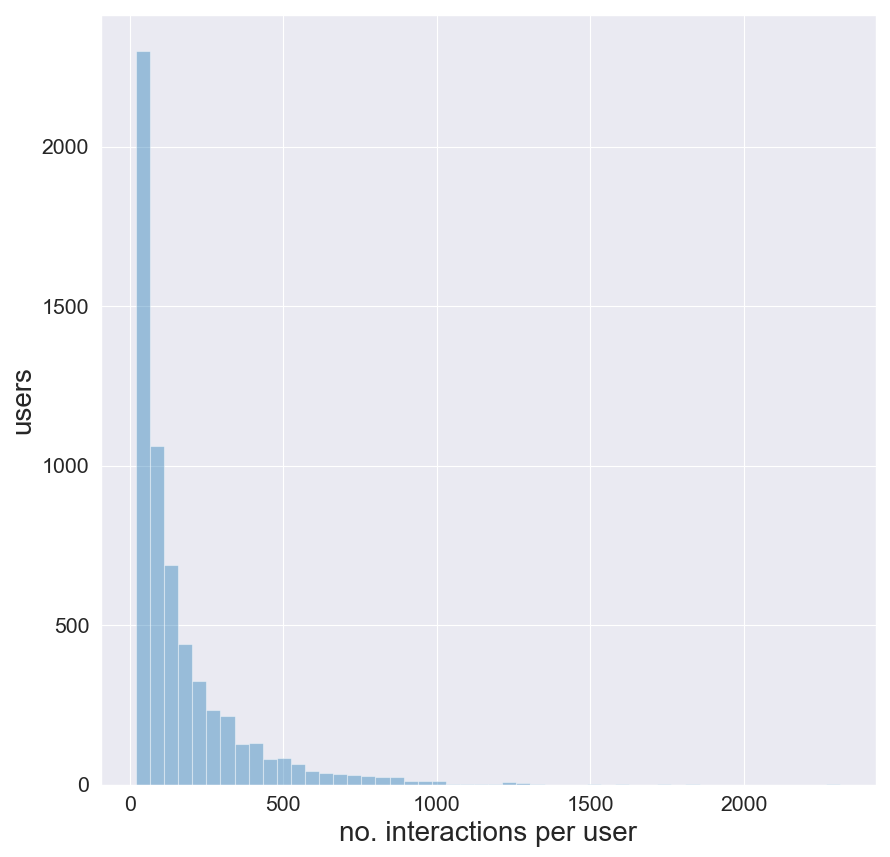
\includegraphics[width=\textwidth]{datasets/Movielens1M_user_interaction_distr.png}
      \caption{MovieLens 1M: distribution of per-user number of interactions}
      \label{fig:ml1m_dist}
    \end{minipage}
    \hfill
    \begin{minipage}{0.48\textwidth}
    \centering
     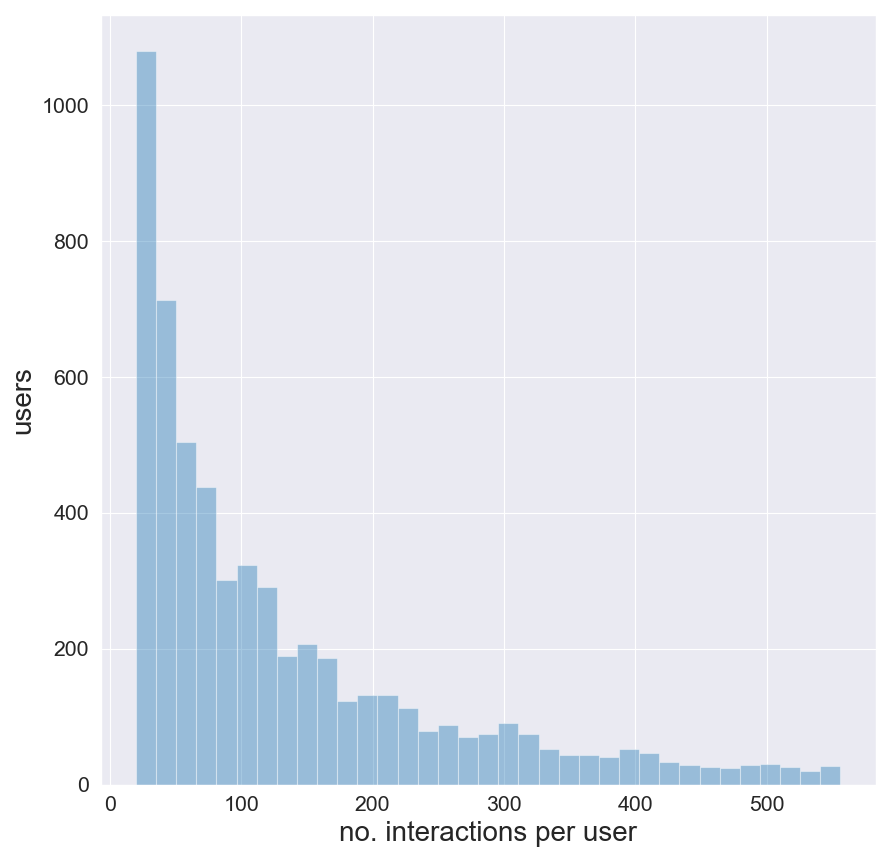
\includegraphics[width=\textwidth]{datasets/Movielens1M_95th_interaction_distr.png} 
     \caption{MovieLens 1M: distribution of 95th percentile number of interactions}
      \label{fig:ml1m_dist_95}
    \end{minipage}
\end{figure}

\subsection{MovieLens 10M}
MovieLens 10M is the other version of MovieLens that we consider in this work. It has just over 10 million interactions from 69878 users rating 10677 items. The matrix density in this version is at 1.34\%. The ratings are explicit in the range $[0.5-5]$ with a step of 0.5. The mean number of interactions per user is 143.11, the maximum is 7359 and the minimum is 20 just like in the MovieLens 1M version. Table \ref{tab:ml10m_stats} summarizes the dataset statistics.

\begin{table}[h!]
    \centering
    \begin{tabular}{c|c}
        \hline
        Interactions & 10000054 \\
        Density & 1.34\% \\
        Users & 69878 \\
        Items & 10677 \\
        Avg. interactions & 143.11 \\
        Min. interactions & 20 \\
        Max. interactions & 7359 \\
        \hline
    \end{tabular}
    \caption{MovieLens 10M dataset statistics}
    \label{tab:ml10m_stats}
\end{table}

\begin{figure}[htbp]
    \begin{minipage}{0.48\textwidth}
    \centering
      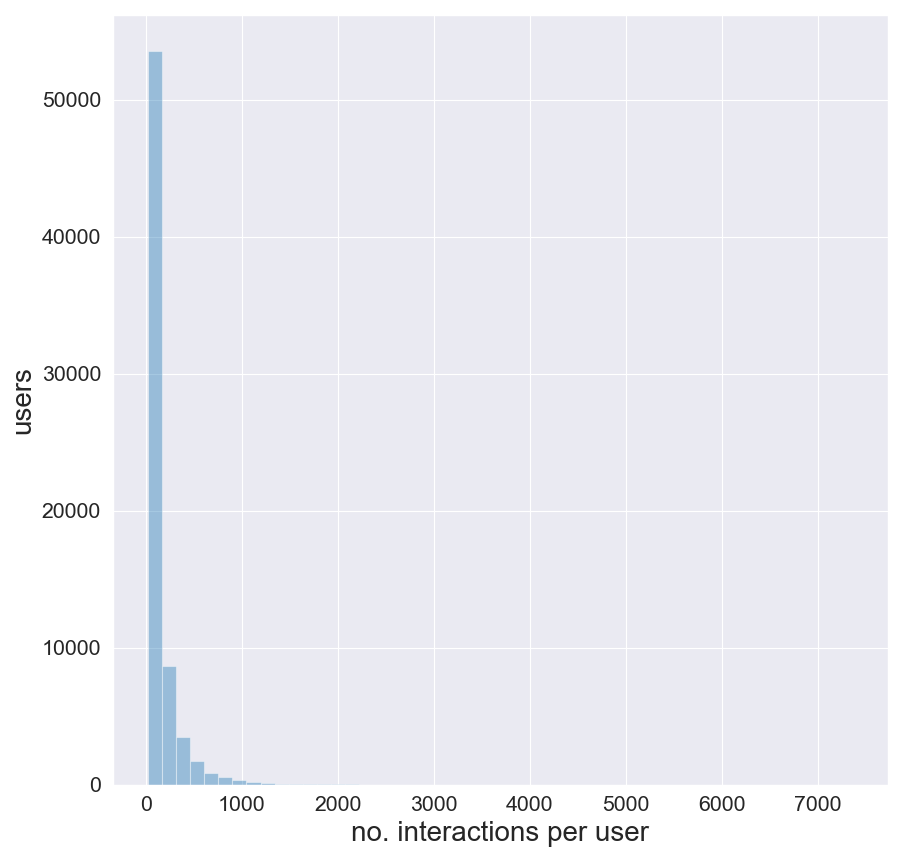
\includegraphics[width=\textwidth]{datasets/Movielens10M_user_interaction_distr.png}
      \caption{MovieLens 10M: distribution of per-user number of interactions}
      \label{fig:ml10m_dist}
    \end{minipage}
    \hfill
    \begin{minipage}{0.48\textwidth}
    \centering
     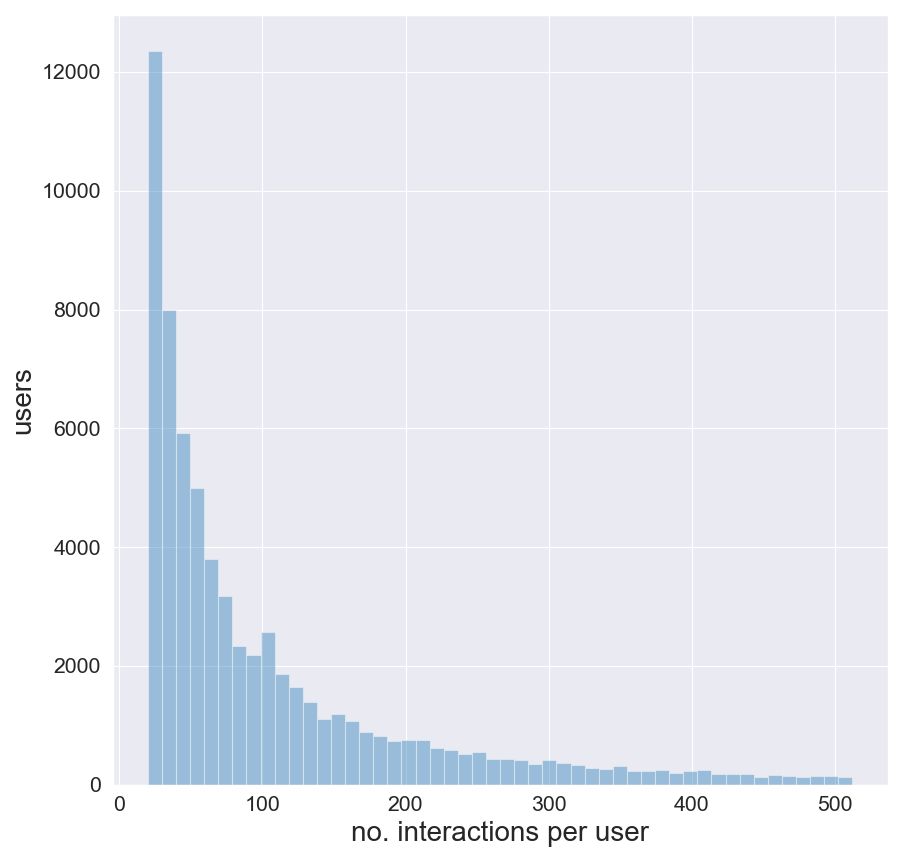
\includegraphics[width=\textwidth]{datasets/Movielens10M_95th_interaction_distr.png} 
     \caption{MovieLens 10M: distribution of 95th percentile number of interactions}
      \label{fig:ml10m_dist_95}
    \end{minipage}
\end{figure}

\section{CiaoDVD}
CiaoDVD dataset\cite{guo2014etaf} is hosted by LibRec\footnote{https://www.librec.net/datasets.html} which is a Java-based library for Recommender Systems. The authors have crawled the entire catalogue of DVDs from the website dvd.ciao.co.uk. The dataset contains ratings in the range $[1-5]$ by 17615 users on 16121 for a total of 72345 ratings. The dataset has a density of 0.025\%, much sparser than all the other datasets we considered. The average number of ratings' per user is 4.11, the minimum is 1 and the maximum number of ratings is 1106.

\begin{table}[h!]
    \centering
    \begin{tabular}{c|c}
        \hline
        Interactions & 72345 \\
        Density & 0.025\% \\
        Users & 17615 \\
        Items & 16121 \\
        Avg. interactions & 4.11 \\
        Min. interactions & 1 \\
        Max. interactions & 1106 \\
        \hline
    \end{tabular}
    \caption{CiaoDVD dataset statistics}
    \label{tab:ciao_stats}
\end{table}

\begin{figure}[htbp]
    \begin{minipage}{0.48\textwidth}
    \centering
      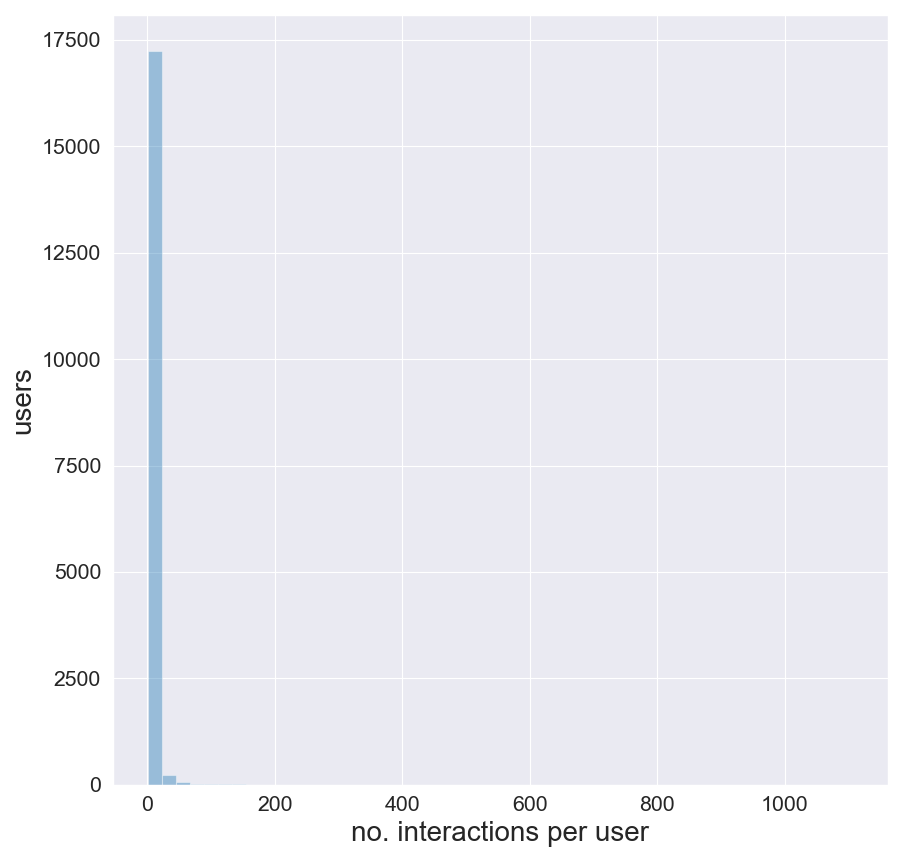
\includegraphics[width=\textwidth]{datasets/CiaoDVD_user_interaction_distr.png}
      \caption{CiaoDVD: distribution of per-user number of interactions}
      \label{fig:ciao_dist}
    \end{minipage}
    \hfill
    \begin{minipage}{0.48\textwidth}
    \centering
     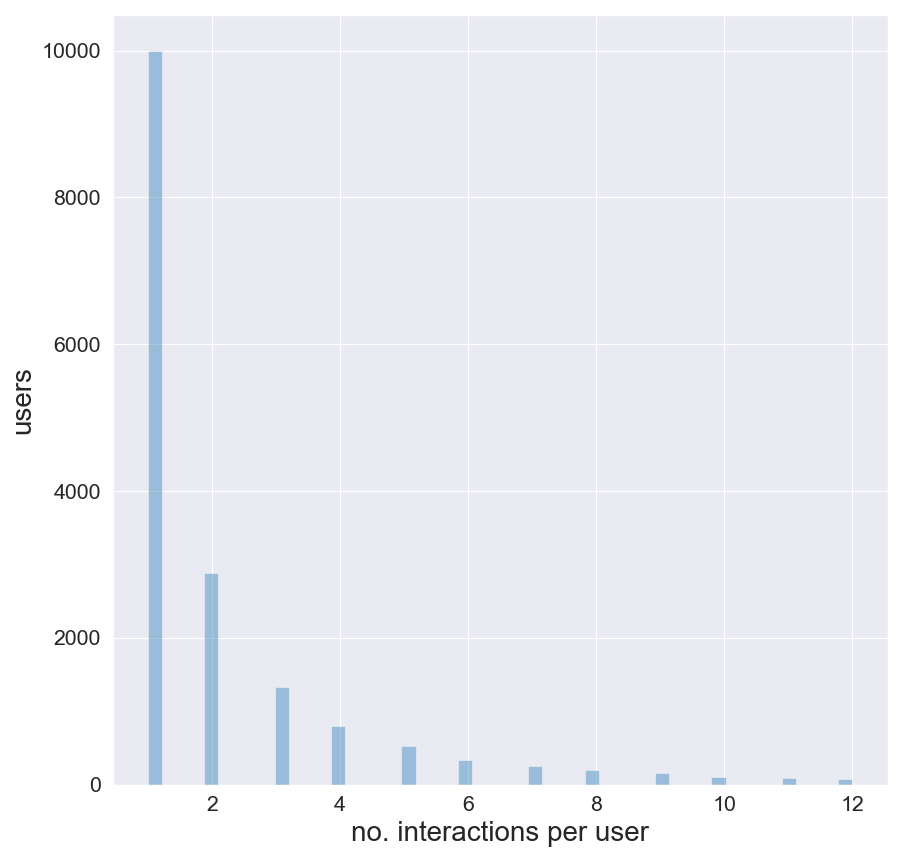
\includegraphics[width=\textwidth]{datasets/CiaoDVD_95th_interaction_distr.png} 
     \caption{CiaoDVD: distribution of 95th percentile per-user number of interactions}
      \label{fig:ciao_dist_95}
    \end{minipage}
\end{figure}

\section{Delicious}
Delicious\cite{Cantador:RecSys2011} dataset is obtained by the Delicious social bookmarking system and release in the 2nd International Workshop on Information Heterogeneity and Fusion in Recommender Systems. It contains tuples of the form (user, bookmark, tag) denoting tags users put to bookmarked URLs. To construct the URM required for testing our algorithms we keep only the pairs (user, bookmark) as \emph{implicit} interactions. There are in total 104799 interactions between 1867 users and 69223 bookmarks. The density of the URM matrix is 0.081\% and the mean number of tagged bookmarks per user is 56.13. This dataset also has users with only one interaction as the minimum number of interactions per user. Table \ref{tab:delicious_stats} summarizes the dataset statistics.

\begin{table}[h!]
    \centering
    \begin{tabular}{c|c}
        \hline
        Interactions & 104799 \\
        Density & 0.081\% \\
        Users & 1867 \\
        Items & 69223 \\
        Avg. interactions & 56.13 \\
        Min. interactions & 1 \\
        Max. interactions & 95 \\
        \hline
    \end{tabular}
    \caption{Delicious dataset statistics}
    \label{tab:delicious_stats}
\end{table}

\begin{figure}[htbp]
    \begin{minipage}{0.48\textwidth}
    \centering
      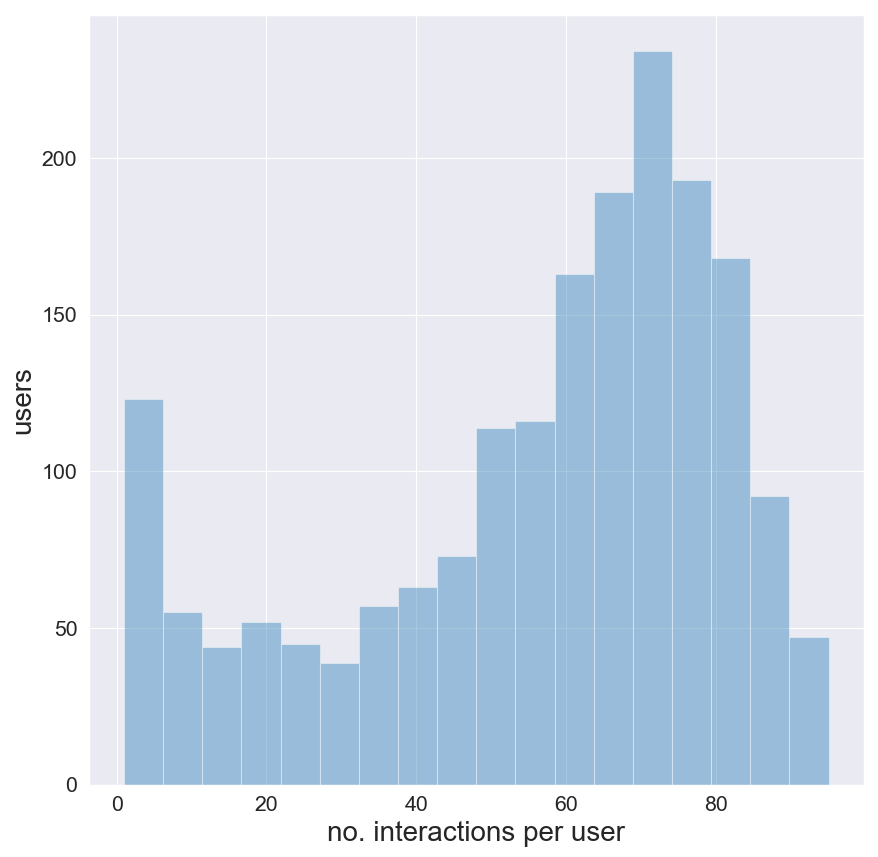
\includegraphics[width=\textwidth]{datasets/Delicious_user_interaction_distr.png}
      \caption{Delicious: distribution of per-user number of interactions}
      \label{fig:delisious_dist}
    \end{minipage}
    \hfill
    \begin{minipage}{0.48\textwidth}
    \centering
     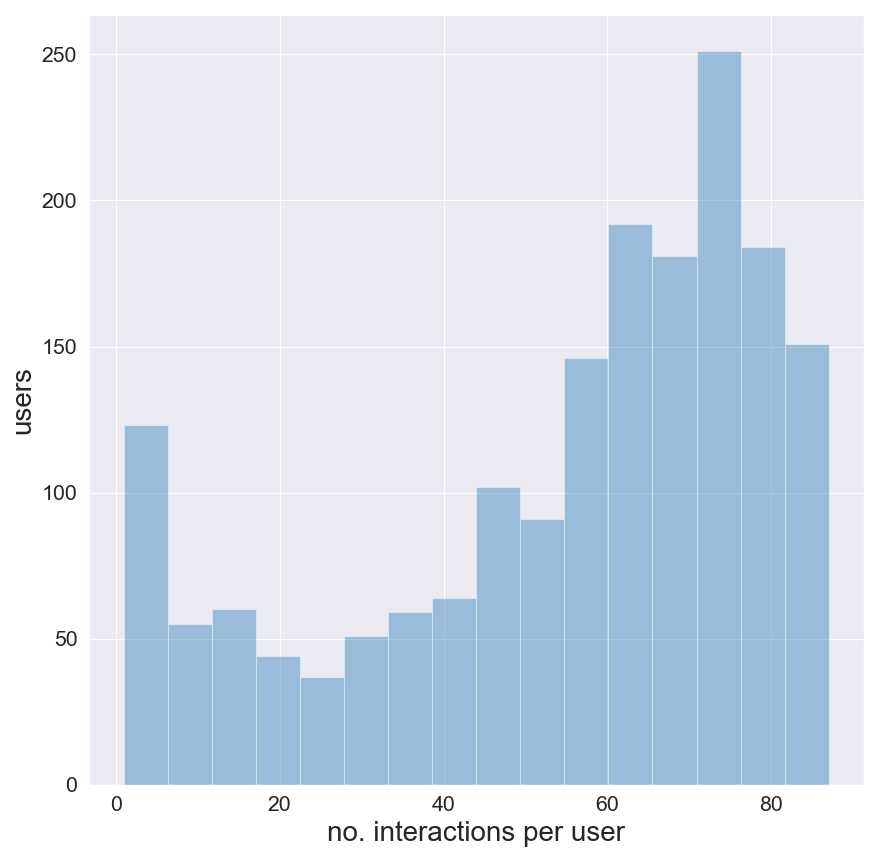
\includegraphics[width=\textwidth]{datasets/Delicious_95th_interaction_distr.png} 
     \caption{Delicious: distribution of 95th percentile per-user number of interactions}
      \label{fig:delisious_dist_95}
    \end{minipage}
\end{figure}

\section{Jester}
Jester\cite{goldberg2001eigentaste} dataset is composed of ratings of 73421 users on 100 jokes. The ratings are in the continuous range $[-10, 10]$ with the score 99 denoting not-rated jokes by respective users. There are around 4.1 million ratings making the resulting URM the most dense we worked with at 56.34\%. The mean number of rated jokes per user is 56.34 with users having rated at least 15 jokes.

Since the ratings are in the range $[-10, 10]$ we preprocess the data in order to get them in a similar format like the other ones. This is especially important from a computational perspective since working with dense matrices brings up memory errors and longer execution times. We shift all ratings in the continuous range $[1-21]$ with 1 meaning a maximum dislike and 21 a maximum like of the joke. We also convert scores of 99 to 0 achieving in this way the sparsification of the resulting URM. We summarize the dataset in Table \ref{tab:jester_stats}.

\begin{table}[h!]
    \centering
    \begin{tabular}{c|c}
        \hline
        Interactions & 4136360 \\
        Density & 56.34\% \\
        Users & 73421 \\
        Items & 100 \\
        Avg. interactions & 56.34 \\
        Min. interactions & 15 \\
        Max. interactions & 100 \\
        \hline
    \end{tabular}
    \caption{Jester dataset statistics}
    \label{tab:jester_stats}
\end{table}

\begin{figure}[htbp]
    \begin{minipage}{0.48\textwidth}
    \centering
      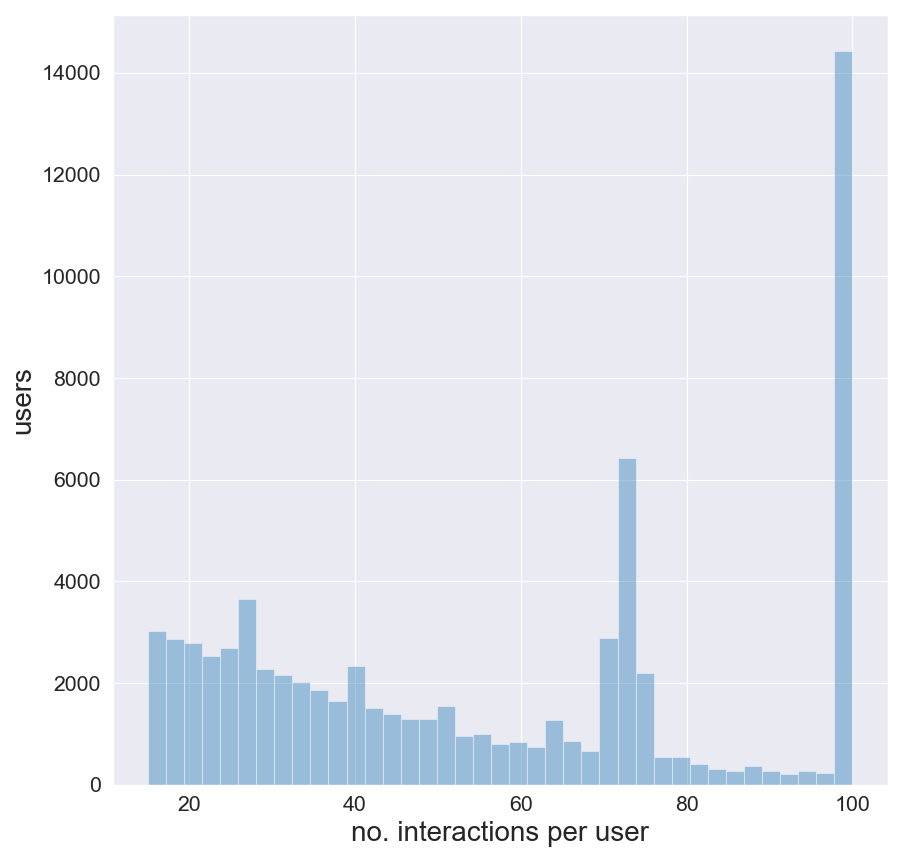
\includegraphics[width=\textwidth]{datasets/Jester_user_interaction_distr.png}
      \caption{Jester: distribution of per-user number of interactions}
      \label{fig:jester_dist}
    \end{minipage}
    \hfill
    \begin{minipage}{0.48\textwidth}
    \centering
     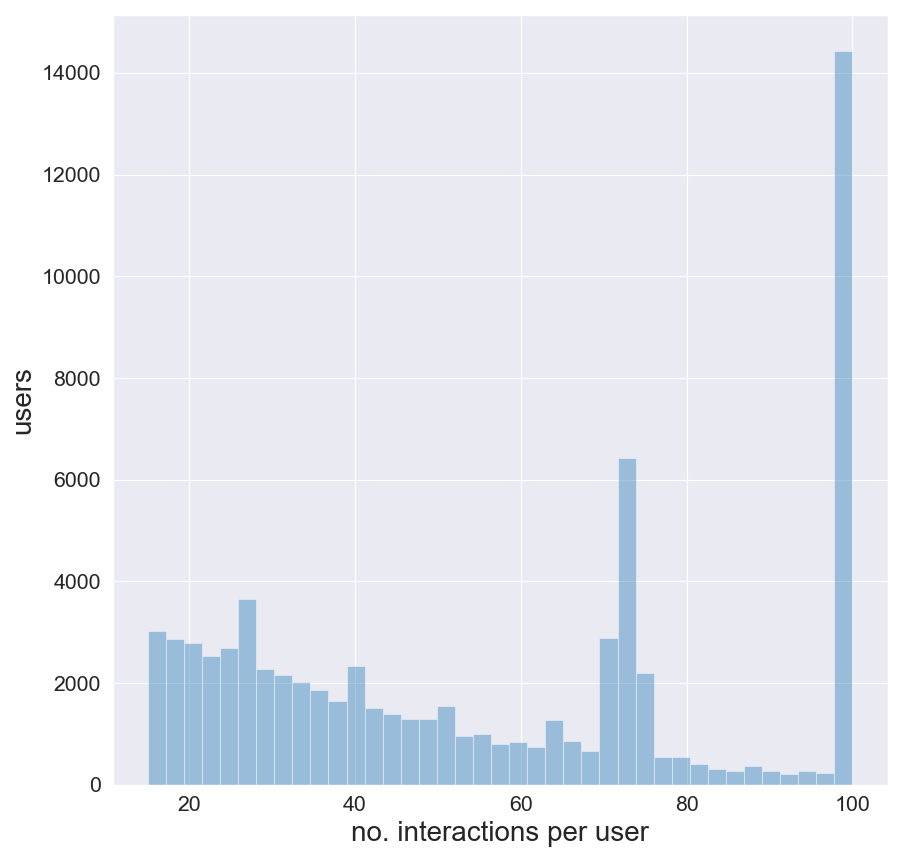
\includegraphics[width=\textwidth]{datasets/Jester_95th_interaction_distr.png} 
     \caption{Jester: distribution of 95th percentile per-user number of interactions}
      \label{fig:jester_dist_95}
    \end{minipage}
\end{figure}

\section{LastFM}
LastFM\cite{Cantador:RecSys2011} is another dataset made available in the 2nd International Workshop on Information Heterogeneity and Fusion in Recommender Systems. It contains music artist listening information from almost 1900 users for 17632 unique artists in the format (user, artist, listeningCount) where \emph{listeningCount} represents how many times the user listened to the specific artist. For our evaluations we consider only the pairs (user, artist) as \emph{implicit} feedback. The URM from this dataset is 0.28\% dense with 92834 pairs. On average a single user has listened to 49.07 different artists with a maximum of 50 and every user has listened to at least 1 artist. Table \ref{tab:lastfm_stats} summarizes the statistical information of LastFM dataset.

\begin{table}[h!]
    \centering
    \begin{tabular}{c|c}
        \hline
        Interactions & 92834 \\
        Density & 0.28\% \\
        Users & 1900 \\
        Items & 17632 \\
        Avg. interactions & 49.07 \\
        Min. interactions & 1 \\
        Max. interactions & 50 \\
        \hline
    \end{tabular}
    \caption{LastFM dataset statistics}
    \label{tab:lastfm_stats}
\end{table}

\begin{figure}[htbp]
    \begin{minipage}{0.48\textwidth}
    \centering
      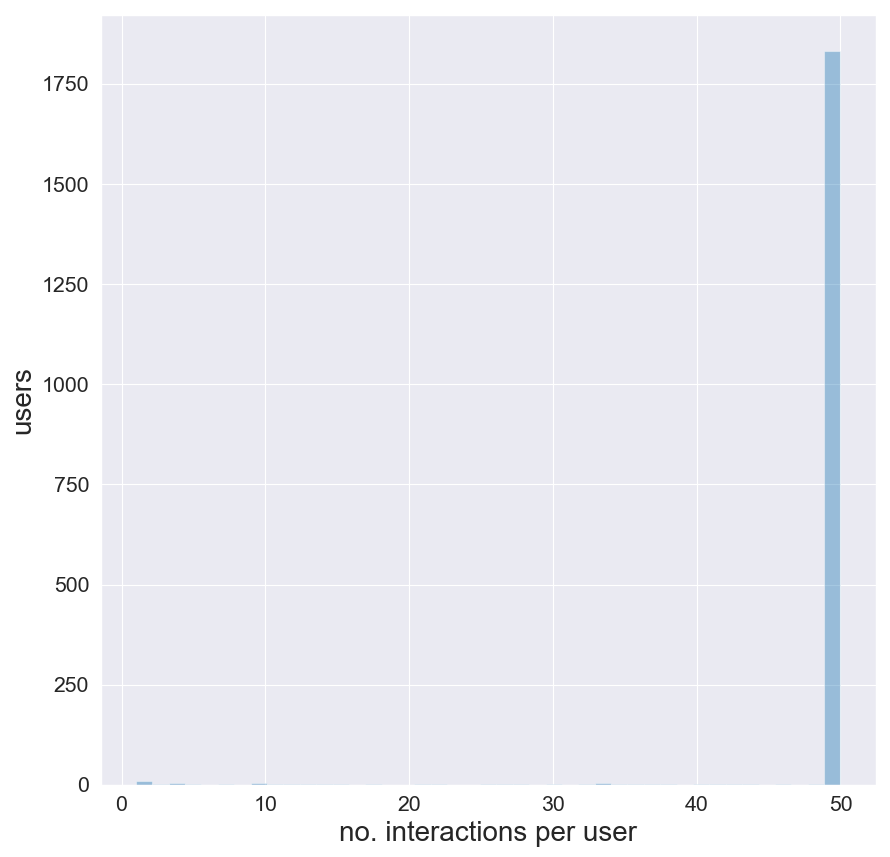
\includegraphics[width=\textwidth]{datasets/LastFM_user_interaction_distr.png}
      \caption{LastFM: distribution of per-user number of interactions}
      \label{fig:lastfm_dist}
    \end{minipage}
    \hfill
    \begin{minipage}{0.48\textwidth}
    \centering
     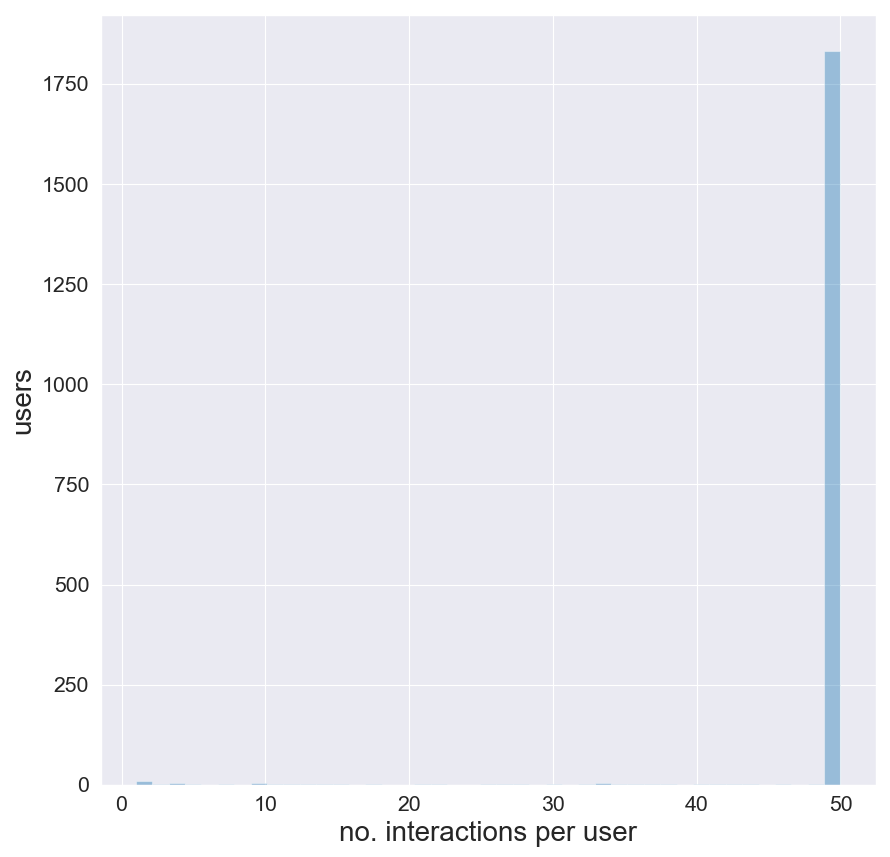
\includegraphics[width=\textwidth]{datasets/LastFM_95th_interaction_distr.png} 
     \caption{LastFM: distribution of 95th percentile per-user number of interactions}
      \label{fig:lastfm_dist_95}
    \end{minipage}
\end{figure}

\section{Book-Crossing}
Book-Crossing\cite{ziegler2005improving} dataset is the result of crawling from Book-Crossing\footnote{www.bookcrossing.com} the 430000 ratings from 78000 users on 186000 books in the range $[1-10]$. Users have rated at least 1 book and on average 5.57 books. This dataset is the sparsest we worked on during this thesis with a sparsity of 0.003\%.

\begin{table}[h!]
    \centering
    \begin{tabular}{c|c}
        \hline
        Interactions & 433670 \\
        Density & 0.003\% \\
        Users & 77804 \\
        Items & 185972 \\
        Avg. interactions & 5.57 \\
        Min. interactions & 1 \\
        Max. interactions & 8524 \\
        \hline
    \end{tabular}
    \caption{Book-Crossing dataset statistics}
    \label{tab:bx_stats}
\end{table}

\begin{figure}[htbp]
    \begin{minipage}{0.48\textwidth}
    \centering
      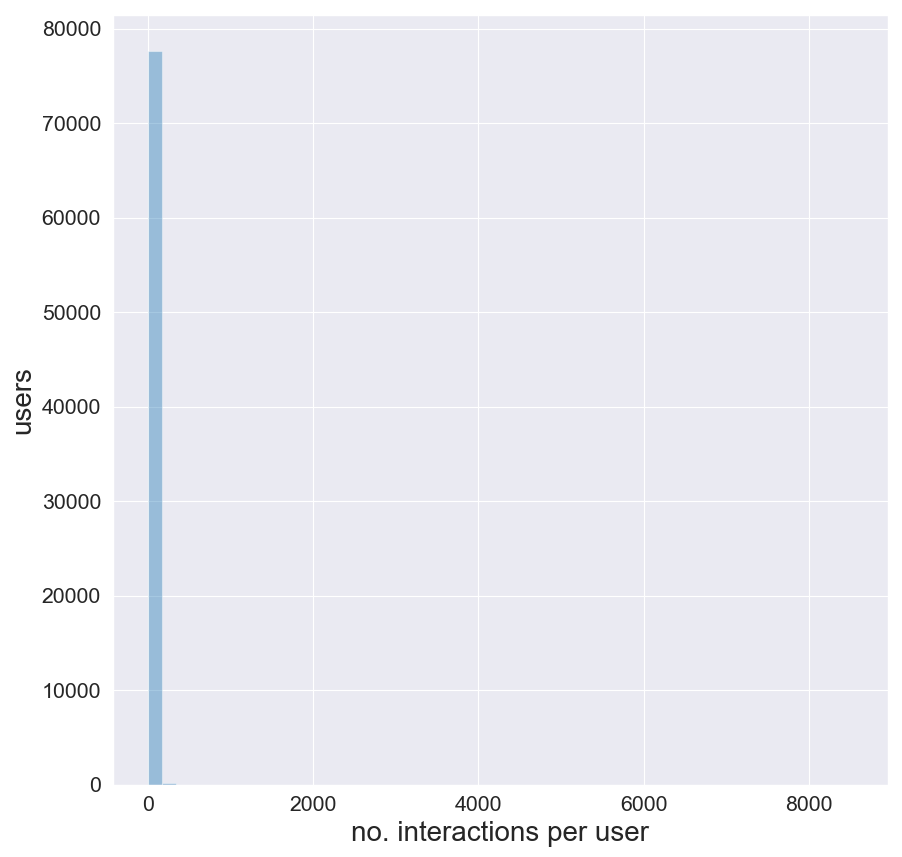
\includegraphics[width=\textwidth]{datasets/Book-Crossing_user_interaction_distr.png}
      \caption{Book-Crossing: distribution of per-user number of interactions}
      \label{fig:bx_dist}
    \end{minipage}
    \hfill
    \begin{minipage}{0.48\textwidth}
    \centering
     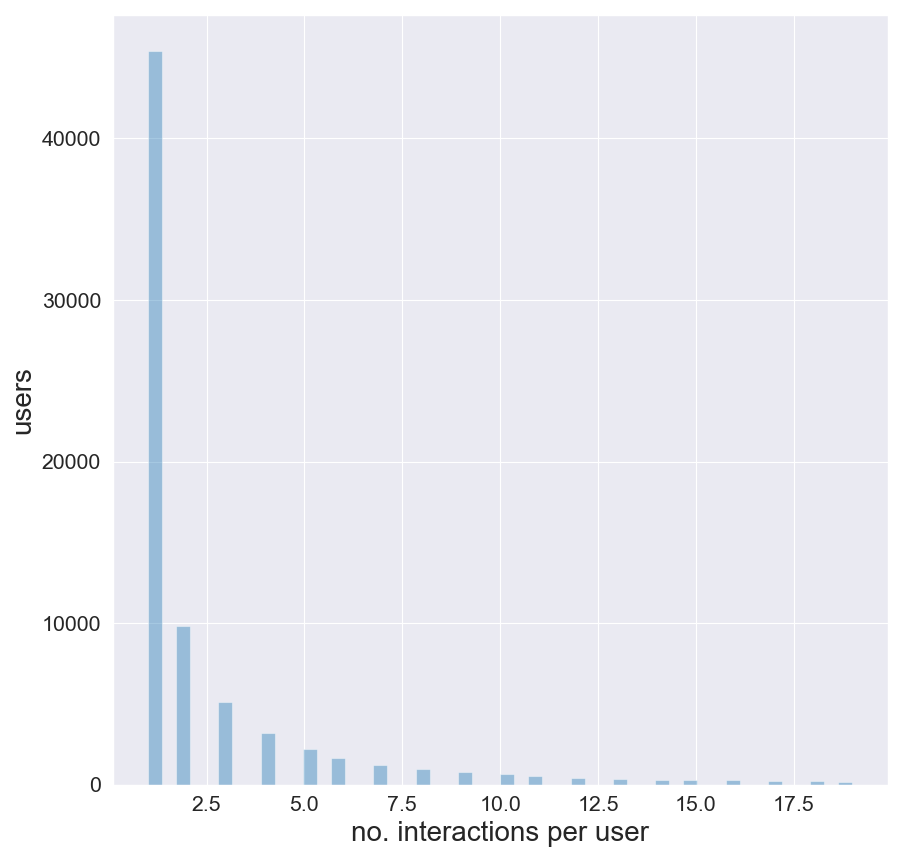
\includegraphics[width=\textwidth]{datasets/Book-Crossing_95th_interaction_distr.png} 
     \caption{Book-Crossing: distribution of 95th percentile per-user number of interactions}
      \label{fig:bx_dist_95}
    \end{minipage}
\end{figure}